% For the map we need to know transmission locations.
% No locations in the telegrams, but "reporting points"

% Urbic site leaked quite some junction numbers
% sweatshop => json => first frontend up and running
% By hand doesn't scale, and OSINT is unrelaible source of the info => mapping

% record telegrams and positions => cross reference via time
% nice mobile box, gps tracker everyone has in their pocket nowadays

% run number is important!

% lofi! Several modes of operation.

% Process Now
%Low coverage => box plus phone
% nice stations => just GPS tracks

% Process in da future
% infer run number!
% just a track, with a nice web front

% Far future => infer as much as possible

%%%%%%%%%%%%%%%%%%%%%%%%%%%%%%%%%%%%%%%%%%%%%%%%%%%%%%%%%%%%%%%%%%%
\begin{frame}[fragile]
  \frametitle{The Problem}
  \framesubtitle{Where the Foxtrot Telegram Was Transmitted}

  \begin{columns}
    \column{.6\linewidth}

    \begin{itemize}
      \uncover<1->{\item{R09Telegram doesn't provide map position data}}
      \uncover<1->{\item{location is identified by arbitrary integer reporting\_point}}
      \uncover<2->{\item{To the Google we go!}}
  \end{itemize}

  \column{.4\linewidth}

  \begin{lstlisting}[basicstyle=\scriptsize]
{
  ...
  "reporting_point":8366,
  "junction":209,
  "direction":1,
  "request_status":2,
  ...
}
  \end{lstlisting}

\end{columns}

\end{frame}

%%%%%%%%%%%%%%%%%%%%%%%%%%%%%%%%%%%%%%%%%%%%%%%%%%%%%%%%%%%%%%%%%%%
\begin{frame}
  \frametitle{OSINT Data}
  \framesubtitle{Or Google Your Own LSA ID's}
  \centering
  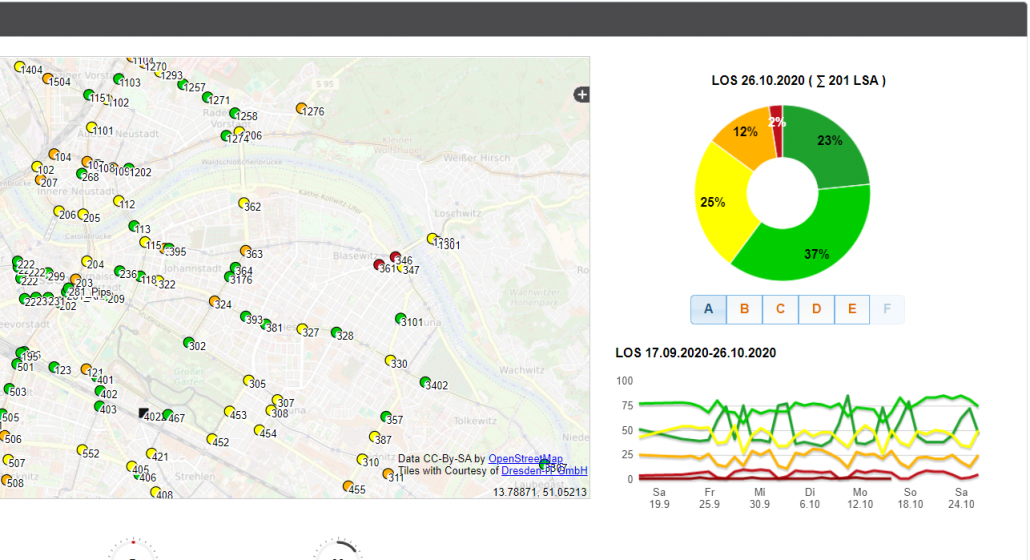
\includegraphics[width=.8\textwidth]{./figs/urbic-osint.png}
\end{frame}

%%%%%%%%%%%%%%%%%%%%%%%%%%%%%%%%%%%%%%%%%%%%%%%%%%%%%%%%%%%%%%%%%%%
\begin{frame}
  \frametitle{Mapping}
  \framesubtitle{JSON Sweatshop, aka Force Your Daughter to Work Day}
  \centering
  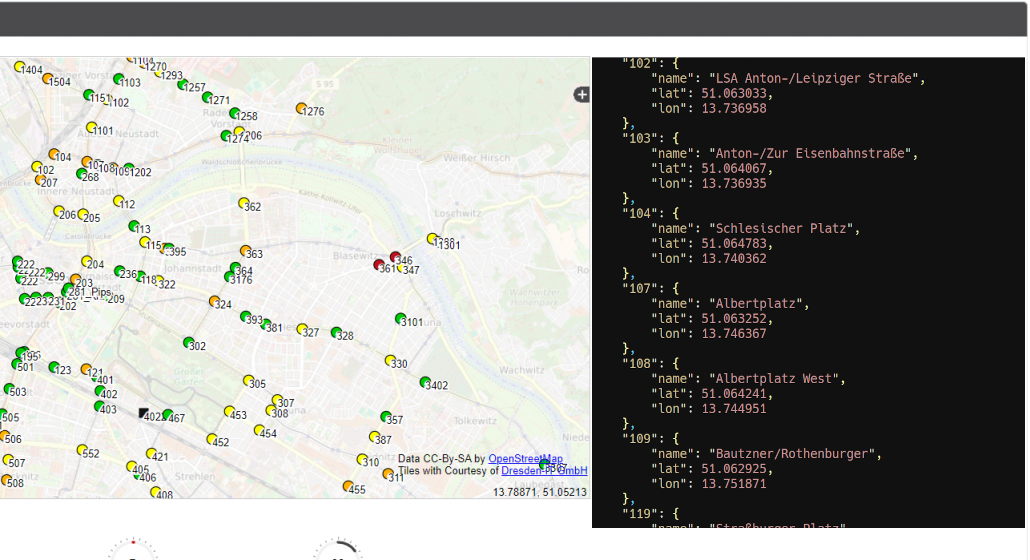
\includegraphics[width=.8\textwidth]{./figs/urbic-osint-json.png}
\end{frame}

%%%%%%%%%%%%%%%%%%%%%%%%%%%%%%%%%%%%%%%%%%%%%%%%%%%%%%%%%%%%%%%%%%%
\begin{frame}
  \frametitle{Mapping}
    \begin{itemize}
      \item "By Hand" doesn't scale too well
      \item OSINT is unreliable source of information
      \item Junction number corresponds to several reporting points
      \item Need a way to correlate telegrams to map location!
    \end{itemize}
    \vspace{20pt}
    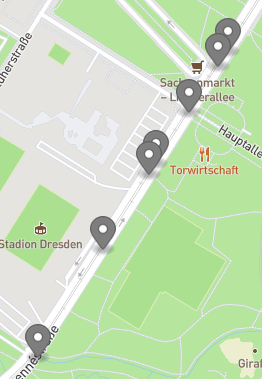
\includegraphics[width=\columnwidth]{./figs/moar_points.png}
\end{frame}

%%%%%%%%%%%%%%%%%%%%%%%%%%%%%%%%%%%%%%%%%%%%%%%%%%%%%%%%%%%%%%%%%%%
\begin{frame}
  \frametitle{Dump DVB: Modern WarFerry}
  \framesubtitle{GPS, Puns and Radio}
  \begin{columns}
    \column{.55\linewidth}
      Telegram Recording:
        \begin{itemize}
      \item SDR with a computer in a tupperware
      \item Running off a powerbank
      \item Wartrammer-40k: filters telegrams
    \end{itemize}
      Location Recording: Phone\\
      Correlation: lofi
    \column{.45\linewidth}
    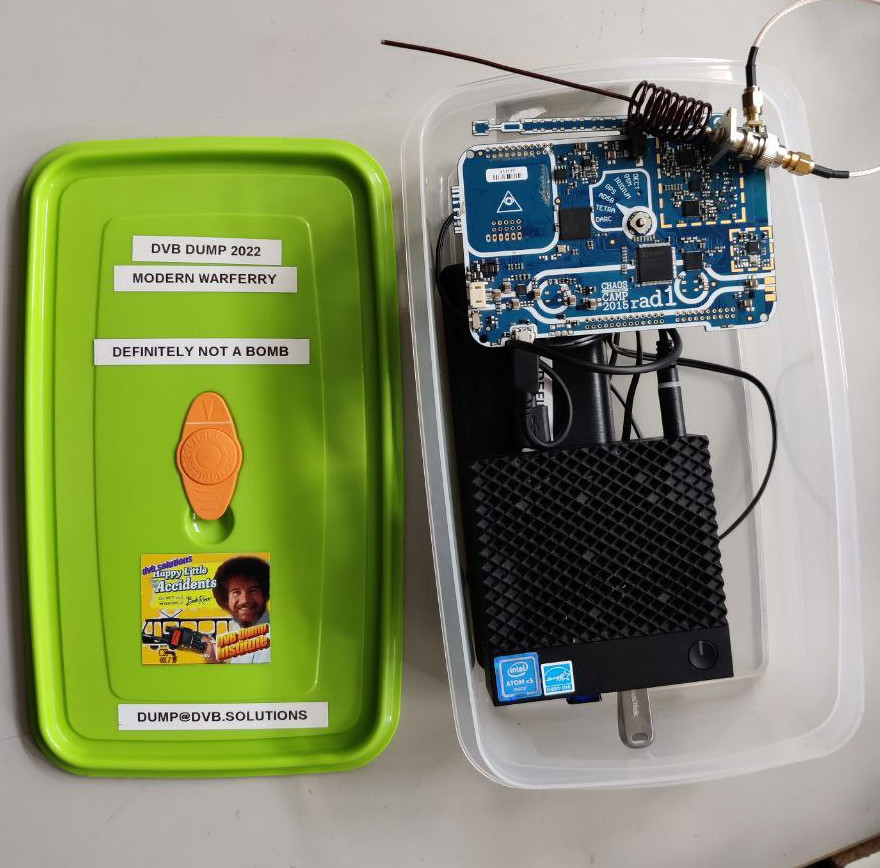
\includegraphics[width=\columnwidth]{./figs/warferry-nude.jpg}
  \end{columns}
\end{frame}

%%%%%%%%%%%%%%%%%%%%%%%%%%%%%%%%%%%%%%%%%%%%%%%%%%%%%%%%%%%%%%%%%%%
\begin{frame}
  \frametitle{Mapping the City}
  \framesubtitle{How It's Done Now}
  \begin{columns}
    \column{.6\linewidth}
    \uncover<1->{
    Bootstraping:
    \begin{itemize}
      \item Go around the city with a warferry
      \item Track your position and line/run number
      \item Correlate the data
    \end{itemize}
  }
  \uncover<2->{
    Decent city coverage by radio stations:
    \begin{itemize}
      \item Go around the city
      \item Track your position and line/run number
      \item Correlate the positions to telegrams from the station
    \end{itemize}
  }
    \column{.4\linewidth}
    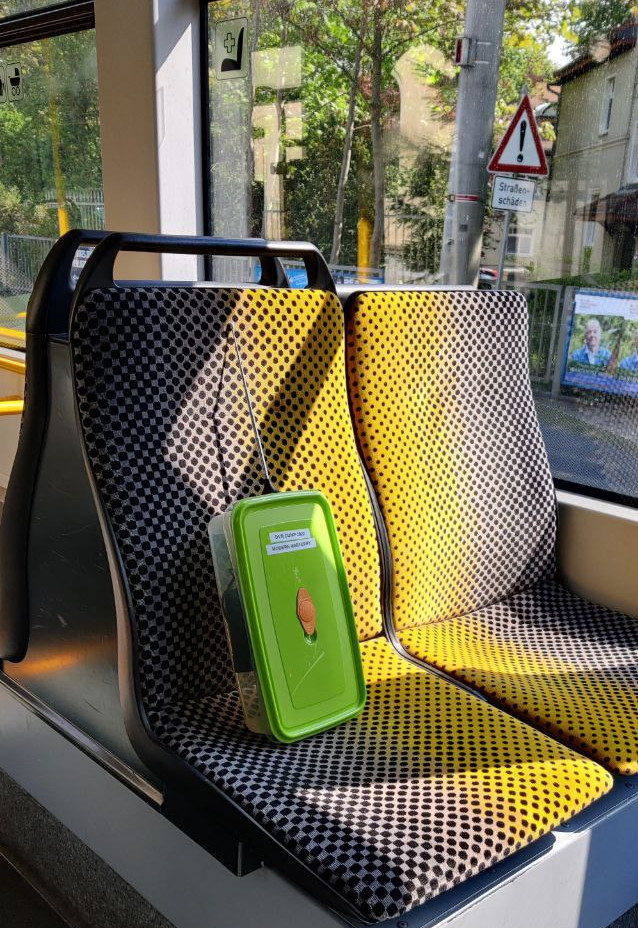
\includegraphics[width=\columnwidth]{./figs/warferry.jpg}
  \end{columns}
\end{frame}

%%%%%%%%%%%%%%%%%%%%%%%%%%%%%%%%%%%%%%%%%%%%%%%%%%%%%%%%%%%%%%%%%%%
\begin{frame}
  \frametitle{Mapping the City, but Better}
  \framesubtitle{Stuff That Still Needs Doing}
  \begin{itemize}
    \item In some cities there is no easy way to get run numbers $\Rightarrow$ inference from reporting point
    \item ``Go around the city'' part sucks
    \item Nice gps track submission web thing (together with line number tracking)
  \end{itemize}
\end{frame}
